% Geometry taken directly from my lectures notes on tight binding in graphene
\newcommand{\alat}{1 cm}
\newcommand{\sqth}{1.73205080757}
\newcommand{\Klen}{2 cm}
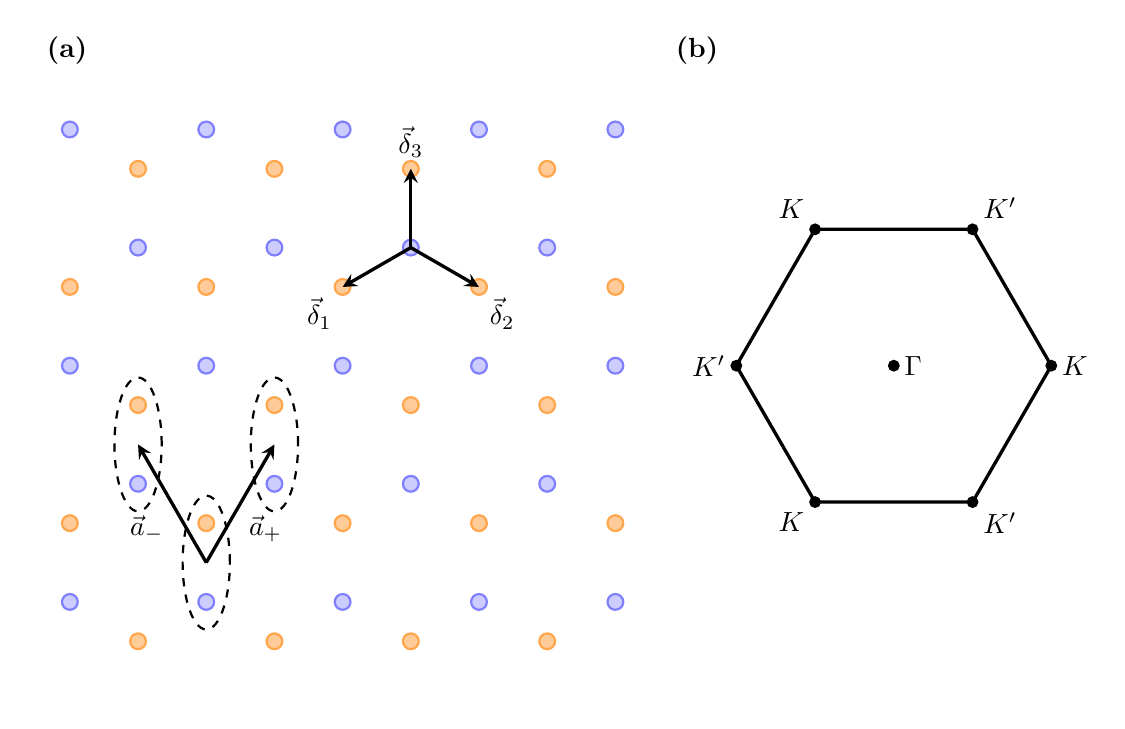
\begin{tikzpicture}															

	% Graphene lattice, sublattices different colors, nearest neighbor vectors and lattice vectors
	\begin{scope}[xshift=-3.5 cm,>=stealth,
		nnarrow/.style={color=black,very thick, ->},					% Nearest neighbor vectors
		A/.style={circle,draw=blue!50,fill=blue!20,
			thick,minimum size=2 mm,inner sep=0pt}, 					% A sublattice dots
		B/.style={circle,draw=orange!70,fill=orange!40,
			thick,minimum size=2mm,inner sep=0pt},						% B sublattice dots
		el1/.style={x radius=.3*\alat,y radius=.85*\alat},				% Style for the ellipse
		el2/.style={dashed,thick}]										% Style for the ellipse draw

		%This scope is clipped to limit the drawn lattice to a square
		\clip (-4cm,-4.25cm) rectangle(4cm,3.75cm);
		% Draw the lattice
		\foreach \ip in {-3,-2,...,3}
			\foreach \im in {-3,-2,...,3}
			{
			\node at (\ip*\sqth*\alat/2-\im*\sqth*\alat/2, \ip*\alat*3/2+\im*\alat*3/2      ) [A] {};
			\node at (\ip*\sqth*\alat/2-\im*\sqth*\alat/2, \ip*\alat*3/2+\im*\alat*3/2+\alat) [B] {};
			}

		% Draw the nearest neighbor vectors
		\draw[nnarrow] (60:\alat*\sqth) -- +(210:\alat) node[anchor=north east]{$\vec{\delta}_1$};
		\draw[nnarrow] (60:\alat*\sqth) -- +(330:\alat) node[anchor=north west]{$\vec{\delta}_2$};
		\draw[nnarrow] (60:\alat*\sqth) -- +( 90:\alat) node[anchor=south     ]{$\vec{\delta}_3$};
		
		% Draw the lattice vectors
		\draw[nnarrow] (240:2*\sqth*\alat) ++(0,\alat/2) --node[circle,anchor=north west]{$\vec{a}_+$} +( 60:\sqth*\alat) ;
		\draw[nnarrow] (240:2*\sqth*\alat) ++(0,\alat/2) --node[circle,anchor=north east]{$\vec{a}_-$} +(120:\sqth*\alat);

		% Ellipses around two atom basis
		\draw[el2] (240:2*\sqth*\alat) ++(0,\alat/2) +(  0,0          ) ellipse[el1];
		\draw[el2] (240:2*\sqth*\alat) ++(0,\alat/2) +( 60:\sqth*\alat) ellipse[el1];
		\draw[el2] (240:2*\sqth*\alat) ++(0,\alat/2) +(120:\sqth*\alat) ellipse[el1];
	\end{scope}

	% Reciprocal space BZ and high symmetry points
	\begin{scope}[xshift=3.5cm,
		BZ/.style={color=black,fill=black,very thick},
		circ2/.style={radius=1.5pt}]

		% Draw the BZ
		\draw[BZ]
			(  0:\Klen) circle[circ2] node[anchor=west      ]{$\bm{K} $} --
			( 60:\Klen) circle[circ2] node[anchor=south west]{$\bm{K'}$} --
			(120:\Klen) circle[circ2] node[anchor=south east]{$\bm{K }$} -- 
			(180:\Klen) circle[circ2] node[anchor=east      ]{$\bm{K'}$} -- 
			(240:\Klen) circle[circ2] node[anchor=north east]{$\bm{K }$} -- 
			(300:\Klen) circle[circ2] node[anchor=north west]{$\bm{K'}$} -- 
			(  0:\Klen);

		% Label the high symmetry points
		\draw[BZ] (0,0) circle[circ2] node[anchor=west]{$\Gamma$};
	\end{scope}

	% (a) and (b) labels
	\node at (-7cm,4cm) {\textbf{(a)}};
	\node at ( 1cm,4cm) {\textbf{(b)}};
\end{tikzpicture}